\documentclass{article}

\usepackage[left=1.5cm,
            right=1.5cm,
            top=2.5cm,
            bottom=2.5cm]{geometry}
\usepackage{hyperref}
\usepackage{fancyhdr}
\usepackage{titling}
\usepackage{verbatim}
\usepackage{amsmath}
\usepackage{graphicx}
\graphicspath{ {./images/} }
\usepackage{longtable}
\usepackage{array}
\newcolumntype{L}[1]{>{\raggedright\let\newline\\\arraybackslash\hspace{0pt}}m{#1}}
\newcolumntype{C}[1]{>{\centering\let\newline\\\arraybackslash\hspace{0pt}}m{#1}}
\newcolumntype{R}[1]{>{\raggedleft\let\newline\\\arraybackslash\hspace{0pt}}m{#1}}
\renewcommand{\arraystretch}{1}

\title{DMML - Assignment 1}
\author{Ishita Pethkar (BMC202128), Siddhant Shah (BMC202171)}
\date{$17^{th}$ March, 2024}

\pagestyle{fancy}
\fancyhead{}
\lhead{\href{https://github.com/SidShah2953/dmml-24-assn-1}{GitHub URL}}
\chead{\thetitle}
\rhead{Ishita Pethkar, Siddhant Shah}

\begin{document}
\thispagestyle{empty}
\maketitle

\tableofcontents
\newpage

\section{Task 1}

\subsection{The Data}
    For this task, we refer to the data set \textit{Customer Churn}, stored at \verb|Data/Customer Churn.csv|. \\
    The data set has the following dimensions: $1000$ rows $\times$ $14$ columns, stored as a \verb|csv| with a size of $71 \operatorname{KB}$. \\
    Overview of the Data Types:
    \begin{itemize}
        \item CustomerID - int64
        \item Age - int64
        \item Gender - object
        \item AnnualIncome - float64
        \item TotalSpend - float64
        \item YearsAsCustomer - int64
        \item NumOfPurchases - int64
        \item AvgTransactionAmount - float64
        \item NumOfReturns - int64
        \item NumOfSupportQueries - int64
        \item SatisfactionScore - int64
        \item LastPurchaseDaysAgo - int64
        \item EmailOptIn - bool
        \item PromotionResponse - object
        \item Churn - bool
    \end{itemize}
    We drop the \verb|CustomerID| column as it is unique and doesn't offer any insights into the Churn.
    To be able to use \verb|AdaBoost|, we need to convert the \verb|object| type columns to numerical column. We do so using the \verb|OrdinalEncoder()| from \verb|scikit-learn|. 

    We then proceed to split the data into training and test sets ($70$-$30$ split), stratifying over \verb|gender|.

\subsection{\texttt{AdaBoost Classifier}}
    We start by finding the ideal hyper-paramters using \verb|GridSearch|, with a \textit{Repeated Stratified $10$-Fold} and \textit{accuracy} as the scoring metric. \\
    We iterate over different values of \verb|n_estimators|, \verb|learning_rate| and \verb|algorithm|. This takes a total time of approximately $150$ seconds.

    \verb|GridSearch| gives us that the ideal values of the hyper-paramters are:
    \begin{itemize}
        \item \verb|algorithm|: 'SAMME'
        \item \verb|learning_rate|: 1e-05,
        \item \verb|n_estimators|: 50
    \end{itemize}
    This configuration gives us an accuracy of $0.5343$.

    We train the final model with these hyper-parameter values, on the training data set. This takes $0.0557$ seconds.

\subsection{\texttt{Random Forest Classifier}}
    We start by finding the ideal hyper-paramters using \verb|GridSearch|, with a \textit{Repeated Stratified $10$-Fold} and \textit{accuracy} as the scoring metric. \\
    We iterate over different values of \verb|n_estimators|, \verb|max_features|, \verb|max_depth| and \verb|max_leaf_nodes|. This takes a total time of approximately $450$ seconds.

    \verb|GridSearch| gives us that the ideal values of the hyper-paramters are:
    \begin{itemize}
        \item \verb|n_estimators|: 200
        \item \verb|max_features|: 'log2'
        \item \verb|max_depth|: 12
        \item \verb|max_leaf_nodes|: 2
    \end{itemize}
    This configuration gives us an accuracy of $0.5252$.

    We train the final model with these hyper-parameter values, on the training data set. This takes $0.1235$ seconds.

\subsection{Model Comparison}
    We make predictions and then evaluate them using a confusion matrix for both models.
    \begin{figure}[h]
        \centering
        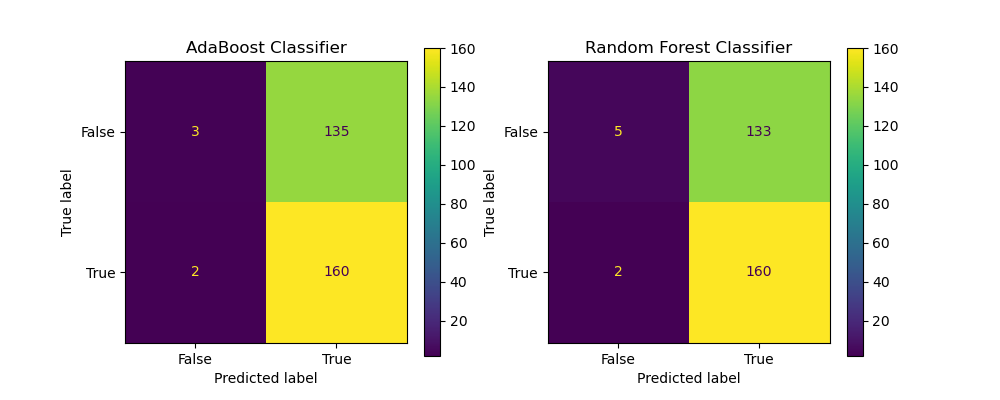
\includegraphics[width=\linewidth]{Task 1.png}
        \caption{Confusion Matrix for Task 1 on Test Data}
        \end{figure}

    As the prediction is a binary value, we compare accuracy, recall \& precision for these two models:
    \begin{table}[h]
        \begin{center}
            \begin{tabular}{|l|l|l|}
                \hline
                Metric &AdaBoost Classifier &Random Forest Classifier \\
                \hline
                Accuracy &0.5433 &0.5500 \\
                Recall &0.9877 &0.9877 \\
                Precision &0.5424 &0.5461 \\
                F1 Score &0.7002 &0.7033 \\
                \hline
            \end{tabular}
        \end{center}
    \end{table}

\newpage

\section{Task 2}

\subsection{Gender Prediction}

\subsubsection{The Data}
    For this task, we refer to the data set \textit{Supermarket Sales}, stored at \verb|Data/Supermarket Sales.csv|. \\
    The data set has the following dimensions: $1000$ rows $\times$ $11$ columns, stored as a \verb|csv| with a size of $80 \operatorname{KB}$. \\
    Overview of the Data Types:
    \begin{itemize}
        \item InvoiceID - object
        \item Branch - object
        \item CustomerType - object
        \item Gender - object
        \item ProductType - object
        \item UnitPrice - float64
        \item Quantity - int64
        \item Tax - float64
        \item Total - float64
        \item PaymentType - object
        \item Rating - float64
    \end{itemize}
    We drop the \verb|InvoiceID| column as it is unique and doesn't offer any insights into the Churn.
    To be able to use these models, we need to convert the \verb|object| type columns to numerical columns. We do so using the \verb|OrdinalEncoder()| from \verb|scikit-learn|. 

    We then proceed to split the data into training and test sets ($70$-$30$ split).

\subsubsection{\texttt{Decision Tree Classifier}}
    We start by finding the ideal hyper-paramters using \verb|GridSearch|, with a \textit{Repeated Stratified $10$-Fold} and \textit{accuracy} as the scoring metric. \\
    We iterate over different values of \verb|max_features|, \verb|max_depth|, \verb|max_leaf_nodes| and \verb|min_samples_leaf|. This takes a total time of approximately $1$ second.

    \verb|GridSearch| gives us that the ideal values of the hyper-paramters are:
    \begin{itemize}
        \item \verb|max_depth|: 9
        \item \verb|max_features|: 'log2'
        \item \verb|max_leaf_nodes|: 10
        \item \verb|min_samples_leaf|: 5
    \end{itemize}
    This configuration gives us an accuracy of $0.5033$.

    We train the final model with these hyper-parameter values, on the training data set. This takes $0.0044$ seconds.

\subsubsection{\texttt{Random Forest Classifier}}
    We start by finding the ideal hyper-paramters using \verb|GridSearch|, with a \textit{Repeated Stratified $10$-Fold} and \textit{accuracy} as the scoring metric. \\
    We iterate over different values of \verb|n_estimators|, \verb|max_features|, \verb|max_depth| and \verb|max_leaf_nodes|. This takes a total time of approximately $180$ seconds.

    \verb|GridSearch| gives us that the ideal values of the hyper-paramters are:
    \begin{itemize}
        \item \verb|n_estimators|: 100
        \item \verb|max_features|: 'log2'
        \item \verb|max_depth|: 6
        \item \verb|max_leaf_nodes|: 10
    \end{itemize}
    This configuration gives us an accuracy of $0.5224$.

    We train the final model with these hyper-parameter values, on the training data set. This takes $0.0917$ seconds.

\subsubsection{Model Comparison}
    We make predictions and then evaluate them using a confusion matrix for both models.
    \begin{figure}[h]
        \centering
        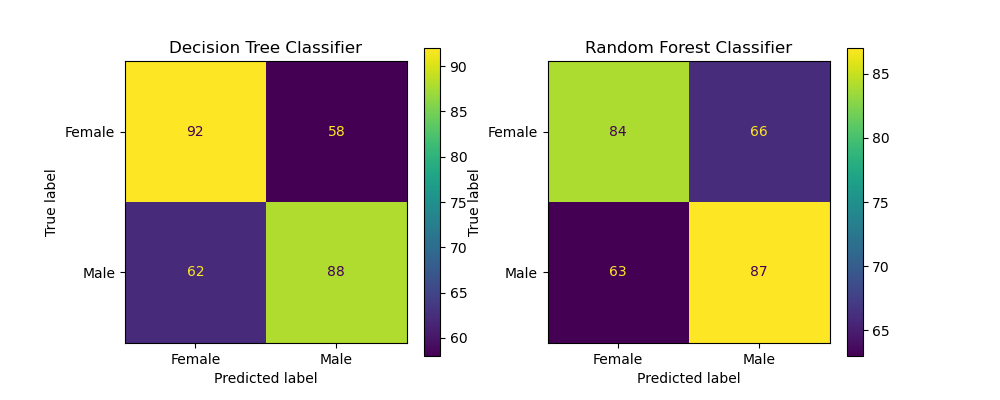
\includegraphics[width=\linewidth]{Task 2A.png}
        \caption{Confusion Matrix for Task 2A on Test Data}
        \end{figure}

    As the prediction is a binary value, we compare accuracy, recall \& precision for these two models:
    \begin{table}[h]
        \begin{center}
            \begin{tabular}{|l|l|l|}
                \hline
                Metric &Decision Tree Classifier &Random Forest Classifier \\
                \hline
                Accuracy &0.6000 &0.5700 \\
                Recall &0.5867 &0.5800 \\
                Precision &0.6027 &0.5686 \\
                F1 Score &0.5964 &0.5743 \\
                \hline
            \end{tabular}
        \end{center}
    \end{table}

\subsection{Ratings Prediction}

\subsubsection{The Data}
    For this task, we refer to the data set \textit{Supermarket Sales}, stored at \verb|Data/Supermarket Sales.csv|. \\
    The data set has the following dimensions: $1000$ rows $\times$ $11$ columns, stored as a \verb|csv| with a size of $80 \operatorname{KB}$. \\
    Overview of the Data Types:
    \begin{itemize}
        \item InvoiceID - object
        \item Branch - object
        \item CustomerType - object
        \item Gender - object
        \item ProductType - object
        \item UnitPrice - float64
        \item Quantity - int64
        \item Tax - float64
        \item Total - float64
        \item PaymentType - object
        \item Rating - float64
    \end{itemize}
    We drop the \verb|InvoiceID| column as it is unique and doesn't offer any insights into the Churn.
    To be able to use these models, we need to convert the \verb|object| type columns to numerical columns. We do so using the \verb|OrdinalEncoder()| from \verb|scikit-learn|. 

    We then proceed to split the data into training and test sets ($70$-$30$ split).

\subsubsection{\texttt{Linear Regressor}}
    As Linear Regression has no hyper-parameters, we run it directly on the training set and get the values of the intercept and coefficients to be as follows:
    \begin{itemize}
        \item Intercept: $6.547981457474257$
        \item Coefficients: \verb|[ 5.66160866e-02 -1.27878875e-02 -1.16013065e-02  8.59907186e-03 1.00556066e-01 -9.26284356e-05 -1.94519715e-03 2.41954803e-02 -7.19095053e-02]|
    \end{itemize}

    This takes $0.0060$ seconds.

\subsubsection{\texttt{Decision Tree Regressor}}
    We start by finding the ideal hyper-paramters using \verb|GridSearch|, with \verb|neg_mean_squared_error| as the scoring metric. \\
    We iterate over different values of \verb|splitter|, \verb|max_depth|, \verb|min_samples_leaf|, \verb|min_weight_fraction_leaf|, \verb|max_features|, and \verb|max_leaf_nodes|. This takes a total time of approximately $75$ seconds.

    \verb|GridSearch| gives us that the ideal values of the hyper-paramters are:
    \begin{itemize}
        \item \verb|max_depth|: 3
        \item \verb|max_features|: 'log2'
        \item \verb|max_leaf_nodes|: 2
        \item \verb|min_samples_leaf|: 2
        \item \verb|min_weight_fraction_leaf|: 0.2
        \item \verb|splitter|: 'random'
    \end{itemize}
    This configuration gives us an MSE of $2.9333$.

    We train the final model with these hyper-parameter values, on the training data set. This takes $0.0029$ seconds.

\subsubsection{Model Comparison}
    As the prediction is a continuous value, we compare the RMSE (Root Mean Squared Error):
    \begin{table}[h]
        \begin{center}
            \begin{tabular}{|l|l|l|}
                \hline
                Metric &Linear Regression &Decision Tree Regressor \\
                \hline
                RMSE &1.7418 &1.7257 \\
                \hline
            \end{tabular}
        \end{center}
    \end{table}

\end{document} % End of document body
